\section{Task definition}

\begin{figure}
    \centering
    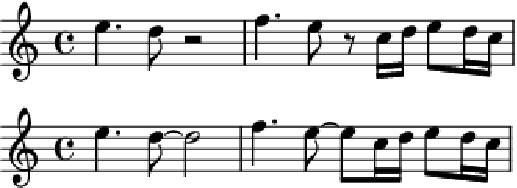
\includegraphics[width=8.1cm]{figs/heuristic_offsets.pdf}
    \caption{
The same note onsets engraved with ground truth~(top) vs. heuristic~(bottom) offsets. 
We argue that onset prediction suffices for producing melody transcriptions that are both recognizable and readable. 
}
 \label{fig:heuristic_offsets}
\end{figure}

\john{You may want to lead here with two definitions: the definition of \emph{melody} (implicitly defined by labels) and the definition of \emph{melody transcription} (in contrast to melody extraction)}

We examine melody transcription, defined here as the task of converting music audio into a \emph{monophonic} (non-overlapping) sequence of \emph{notes} which constitute its melody. 
A note canonically consists of an onset time, a musical pitch, and an offset time, though here (and as in~\cite{laaksonen2014automatic}) we disregard offsets for several reasons. 
First, accuracy of onsets has been found to be far more important to human perception of transcription quality than accuracy of offsets~\cite{ycart2020investigating}. 
Second, in our dataset (which represents a crowdsourced proxy in lieu of a precise definition of melody), a heuristically-determined offset is identical to the ground truth offset for $89\%$ of notes.\footnote{The heuristic we adopt sets the offset of one note equal to the onset of the next, i.e., it assumes the melody is legato.}
Finally, we argue intuitively that onsets and pitches suffice for both recognizing and reading melodies---see~\Cref{fig:heuristic_offsets} for an example. 

Formally, the task of melody transcription is to convert music audio $\bm{a}$, sampled at rate $f_s$, into a list of notes $\bm{y}$, where a note $y_i$ is a pair of onset time $t_i$ and musical pitch $n_i$. Hence, 
\begin{align*}
    \bm{a} &= a_1, \ldots, a_S, \text{where}~S = Tf_s \\
    \bm{y} &= y_1, \ldots, y_N, \text{where}~y_i = (t_i, n_i).
        %&&t_i \leq T, \text{and} n_i \in \{\text{A0}, \ldots, \text{C8}\}
\end{align*}
To handle the high dimensionality of audio, transcription algorithms typically extract features $\bm{X}$ (a matrix) from audio, which are sampled at $f_k \ll f_s$:
\begin{align*}
    \text{Extract}(\bm{a}) = \bm{X} = \bm{x}_1, \ldots, \bm{x}_M, \\ 
    \text{where}~M = Tf_k~\text{and}~\bm{x}_i \in \mathbb{R}^d.
\end{align*}
Hence, in practice, our goal is to build a transcription method 
$f : \bm{X} \mapsto \bm{y}$.
% $f$ which maps features $\bm{X}$ to notes $\bm{y}$. 

\subsection{Evaluation}
\label{sec:eval}

\todo{Draw distinction from frame-based metrics used to evaluate melody extraction}
% CHRIS: This maps cleanly onto our contributions (standardized evaluation and new datasets), but may be too snarky for paragraph 2
%Finally, we argue that a historical focus on the important but disparate task of melody \emph{extraction}---detecting the time-varying fundamental frequency of the melody as opposed to its discrete notes---has led to a lack of work on transcription and systemic issues in evaluation.

\john{Leading with an MIR implementation of F1 is a little confusing, especially since it is not typically applied to this task (you are defining the task, right?)}
To evaluate a melody transcription method $f$, 
we incorporate a standard approach~\cite{raffel2014eval} for computing an \fone{} score between reference $\bm{y}$ and estimate $f(\bm{X})$. 
This approach---shown in~\cite{ycart2020investigating} to correlate with human perception---scores estimates by aligning their onsets to the reference onsets with $50$ms of tolerance, and then computes a standard \fone{} score, where an estimated note is treated as correct if it is the same pitch as the matched reference:
\begin{equation*}
    \text{Score} : f(\bm{X}), y \mapsto [0, 1].
\end{equation*}

\john{This adjustment seems to be needed because of the nature of the annotations (next section) but it's pretty confusing introducing it before that discussion}
In other transcription settings, evaluation conventionally requires that estimates match the octave of the reference. 
In melody transcription, where transcriptions are prone to be performed on different instruments or by vocalists with different ranges, predicting the correct octave is less critical for downstream use. 
Previous evaluations for melody extraction gave full credit for estimates with the right pitch class (see~\cite{poliner2007melody} for a summary), however we argue that \emph{relative} octave information is important for transcription accuracy. 
Hence, we modify the evaluation criteria to allow models to achieve a perfect score if they produce the correct notes but are off by a fixed octave shift:
\begin{equation*}
    \max_{i \in \mathbb{Z}} \text{Score}(\text{OctaveShift}(f(\bm{X}), i), \mathbf{y}).
\end{equation*}